\documentclass{article}
\def\npart {2}
\def\nterm {LMS Summer School}
\def\nyear {2021}
\def\nlecturer {Various}
\def\ncourse {Colloquia}

\input{header}

\begin{document}
  \maketitle

\section{Markov Numbers and the free group on two generators - Caroline Series.}

We are going to talk about three binary tree and the connections between them.

A Markov number is a solution to,
$$ x^2 + y^2 + z^2 = 3xyz $$
If we set $x=y=z=1$ and that's a solution. Let's not worry about negative solutions as here is another $(-x, -y, z)$. \\

Suppose $x, y_1, z_1$ is a solution you get,
$$ z^2 - 3xy_1z_1 + y_1^2 + z_1^2 = 0 $$
and so $x + x' = 3y_1z_1$. If we have $(x, y_1, z_1)$ we can get $(3y_1z_1 - x, y_1, z_1)$. We could permute any of these. \\

\begin{nthm}
  If we start with a solution, we can carry on permuting, we can get all the solutions,
  $$ (x, y, z) \to (3yz - x, y, z) $$
\end{nthm}
\begin{proof}
  Start with $(x, y, z)$, and let $(1, 1, 1)$ and thenget a load of solutions. We can now put these around the vertices of a binary tree.
  \begin{figure}[!ht]
    \centering
    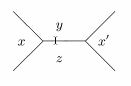
\includegraphics{./figures/L1.1}
  \end{figure}
  and we can do this again, to get a load more solutions,
  \begin{figure}[!ht]
    \centering
    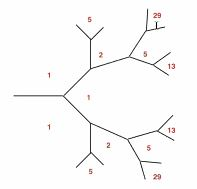
\includegraphics{./figures/L1.2}
  \end{figure}
  Let's now prove that this is all of them, \\
  Say it is special if two of $x, y, z$ are equal. The only special solutions are $(1, 1, 1)$ and $(1, 1, 2)$. Say $x = y$ and then $2x^2 + z^2 = 3x^2z$. Hence $x^2|z^2$ and so $z = kx$ and so $2 + k^2= 3kx$ so $k|2$ and so $k = 1$ or $2$.\\
  \textbf{Step 2:}
  Show that if $(x, y, z)$ is a solution with x < y < z if x' = 3yz - x and x > y > x'.
  \textbf{Step 3:} Take any non-special $x > y > z$ surrounding $V$ and draw it's local tree with arrows. By step 2, there is an outgoing arrow from $x$ to $x'$.
  \textbf{Claim:} The other two arrows at $V$ point to $V$. \\
  This follows from a change of variables, $\xi + \eta+\zeta = 1$ and so again, $\xi + \xi'=1$ and for the other variables. Hence $\xi > \xi'$ and so $\xi > \frac{1}{2}$. But then, $\eta < \frac{1}{2}$ and $\zeta < \frac{1}{2}$, which means that $\eta < \eta'$ and $\zeta < \zeta'$, so the arrows point to $V$.\\
  \textbf{Step 4:} From each non-special vertex there exists
\end{proof}

There is a conjecture that says,
\begin{conjecture}
  Suppose $x > y > z$ and $x > \hat y > \hat z$ are both solutions to Markov equations, then $y = \hat y$ and $z = \hat z$
\end{conjecture}
The conjecture has been checked up to numbers 140 digits long.
\begin{thm}
  The uniqueness conjecture  is truw if the largest number $x$ is the triple of the form $kp^n$ whiere $p$ is prime and $k \le 10^35$
\end{thm}
A simpler proof is given in 2005 about $x$ being a prime power.

\subsection{Free Group on 2 generators}
A free group of two generators, $F_2$, every element is a product of $a$, $a^{-1}$, $b$ and $b^{-1}$. A string of these is called a word, there are no relations expect the identity relation.\\

A generator pair $(\a, \b) \in F_2$ such that every $g \in F_2$ can be written in terms of $\a^{\pi}$ and $\b^{\pm}$. You can get a new generator pair by inverting one generator or by conjugating.

\begin{nthm}
  Every generator pair can be obtained in this way starting from $(a, b)$.
\end{nthm}

A word $w$ which we can find a $v$ such that they are generators are called primitive. We want all of the primitives of our group. We don't want conjuages so we assume that $w$ isn't cyclically reduced.
\begin{align*}
  w = e_1e_2\dots e_n\\
  e_1^{-1}we_1 = e_2e_3\dots e_ne_1
\end{align*}

He shows that after cycliv permutations and cancelling, then if $(\a, \b)$ is a generator we can just and shorten. For Example take, $(ab^2abab^2, ab^2)$ can be reduced to $(a, b)$.\\

We can now put these around our binary tree. Across an edge we have a generator pair.
\begin{figure}[!ht]
  \centering
  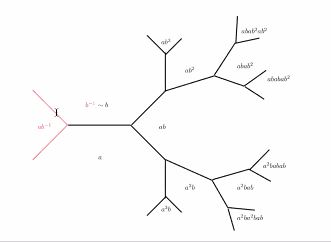
\includegraphics{./figures/L1.4}
\end{figure}
We have generator pairs opposite eachother. We have some fascinating patterns called Sturmian sequences. There is every primite element is represented once and the otheres just have negative exponents.\\

Another proof uses albelianisation of $\Z^2$. If $w \in F_2$ and map it to $\psi (w) = (m, n) \in \Z^2$.We assume everything is commutative and so we can have $\hat w = a^mb^n$. We also note that, $\psi(w^{-1}) = -\psi(w)$ and $\psi(w) = \psi(w')$.\\

\begin{nthm}
  Any primitive element of $F_2$ maps to a relatively prime pair. If $w'$ is another primitive element with $\psi(w') = \psi(w)$, then they are conjuage.
\end{nthm}

What it's telling us that the rationals are an equivilence class around a tree. We shall now look at Farey tree. \\

We say two rationals $\left(\frac{p}{q} \text{ and } \frac{r}{q}\right)$ are neighbours if $ps - rq = \pm 1$. This then means that,
$$ \frac{p}{q} + \frac{r}{s} = \frac{p+r}{q+s} $$
this is called a farey sum and so,
$$ \frac{p}{q} < \frac{p + r}{q + s} < \frac{r}{s} $$
Using the euclidean algorithm it is not hard to show that all positive rationals can be reached this way starting at $\frac{1}{0}$ and $\frac{0}{1}$.
\begin{figure}[!ht]
  \centering
  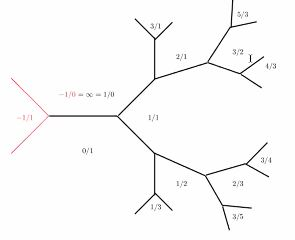
\includegraphics{./figures/L1.5}
\end{figure}
We can just add as we go around and now we have all of the rationals.
We just go around and multiply the trees.\\

Finally we make the connection. Consider elements of $SL(2, \C)$ which all have determinant 1. Now we can consider the trace and it's invariant under conjigation. There are some other polynomial identities. They use the commutator and -2 and we can simplify things nicely,
$$ Tr A Tr B Tr AB = (Tr A)^2 + (Tr B)^2 + (Tr AB)^2 $$
and so we divide by three and get the markov equation. We can also consider $Tr AB^{-1}$ and get that $z + z' = 3xy$. Now it suffices to show that there exists these matrices. Let,
$$ A = \begin{pmatrix}
  1 & 1 \\ 1 & 2
\end{pmatrix} \qquad B = \begin{pmatrix}
  1 & -1 \\ -1 & 2
\end{pmatrix} $$

Now take the tree of generators of the free group and then put them into the Neilson tree and replace $W$ bt $Tr \frac{W}{3}$.\\

\begin{thm}
  The tree of Markov number is found from the three of traces of the above matrices by dividing all entries by 3 and starting the triple $(1, 1, 1)$.
\end{thm}

\subsection{Tree of Traces}
We used the tree of traces and got the special numbers. Why don't any old matrices work? We can sub in and do some generators and find it's trace.

\begin{nlemma}
  Given any triple of complex numbers $(x, y, z)$ there are matrices $A, B \in SL(2, \C)$ so that,
  $Tr A = x$, $Tr B = y$ and $Tr AB = z$
\end{nlemma}
\begin{proof}
  We take,
  $$ A = \begin{pmatrix}
    x & -1 \\ 1 & 0
  \end{pmatrix} \qquad B = \begin{pmatrix}
    0 & \zeta \\ \zeta^{-1} & y
  \end{pmatrix}$$
  where $z = \zeta + \zeta^{-1}$
\end{proof}

and so now we just run through the tree and images of primitive elements. Some questions have been asked is, is the group generated by $A$ and $B$ free? If not, is it discrete?

Are the corresponding groups finite? If we look at the following,
\begin{figure}[!ht]
  \centering
  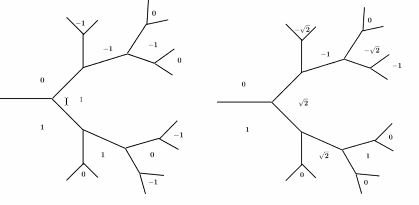
\includegraphics{./figures/L1.6}
\end{figure}

You can see that you won't get past $0$ and $1$ for the first. Then in the second, taking $\sqrt 2$, we can't more values than we have. If a group had generators $0$, $1$ would it be finite? So we now consider $SU(2)$,
$$ M = \begin{pmatrix}
  a & b \\ \overline{a} & \overline{b}
\end{pmatrix} $$
and they are unitary. These basically give us stereographic projections, it didn't preserve distance, but it does for angles. if we rotate our stereographic sphere, we get an angle preserving map. This then gives us $SU(2) \subset SL(2, \C)$. This gives us a mobius transformation. Thn if we consider,
$$ \begin{pmatrix}
  e^{i \frac{\theta}{2}} & 0 \\
  0 & e^{-i \frac{\theta}{2}} \\
\end{pmatrix} $$
We get the trace as just $2\cos \frac{\theta}{2}$. Then out pops $0, 1, \sqrt 2$.

\begin{nthm}
  With one exception, every finite tree is associated to a regular solids, and correspeonds to finite representations to $F_2 \to S(U)$ with finite image. The exception is the dihedral group.
\end{nthm}

The other regular solid is the icosohedron, hence giving the icosohedral group. The sphere is coverd with twenty copies of the a equilateral triangle of angle $\frac{\pi}{5}$. This then moves forward with subgroups generated by rotations of orders $2, 3$ and $5$. So we expect to get a finite tree starting from the values, $2\cos \frac{\pi}{2} = 0$, $2\cos \frac{\pi}{3} = 1$ and $2\cos \frac{\pi}{5} = \omega$ and after some algebra we get that $\omega - \omega - 1 =0$ and hence after some algebra we have finite values.

\section{A Glimpse of Tropical Geometry - Felipe Ricon, QMUL}

Resources - \textit{Introduction to tropical Geometry (Book), First Steps in Tropical Geometry (Article)}

\begin{ndefi}[Tropical Semiring]
  The tropical semiring is,
  $$ \overline{\R} = (\R \cup \{\infty\}, \oplus, \odot) $$
  where,
  $$ \oplus := \min \qquad \odot := + $$
\end{ndefi}

\begin{eg}
  $$ 3 \oplus 5 = 3 \qquad 4 \odot 7 = 11 $$
  $$ \infty \oplus a = a \qquad 0 \odot a = a $$
\end{eg}


$\overline \R$ is an idemoptent remiring as there are no additive inverses.
$$ a \odot (b \oplus c) = a \odot b \oplus a \odot c $$
but things like,
$$ 2 \oplus x = 5 $$
doesn't have a solution in our semiring. But addition is idempotent,
$$ a \oplus a  = a $$
\begin{eg}
  $(x \oplus y)^3 = x^3 \oplus x^2 \odot y \oplus x \odot y^2 \oplus y^3 \equiv x^3\oplus y^3$
\end{eg}

\noindent
Denote $\overline \R [x_1, \dots, x_n]$ the semiring of the tropical polynomials on the variables $x_1, \dots, x_n$.

\begin{eg}
  $f(x) = x^2 \oplus 1 \odot x \oplus 4$
  which then we can plot,
  \begin{figure}[!ht]
  \centering
  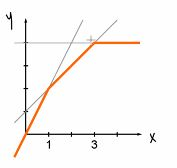
\includegraphics{./figures/L2.1}
  \caption{A graph of $f(x) = (x \oplus 1)\odot (x \oplus 3$}
  \end{figure}

  we note we can factor them as,
  $$ f(x) = (x \oplus 1)\odot (x \oplus 3) $$
  and where we factor it is where the graph bends.
\end{eg}

\newpage
\begin{nthm}[Fundemental Theorem of Algebra]
  If $f(x)\in\overline\R [x]$ has degree $d$ then,
  $$ f(x) \equiv c\odot (x\oplus a_1)^{m_1} \odot (x\oplus a_1)^{m_2} \odot\dots\odot (x\oplus a_r)^{m_r} $$
  where $a_1, \dots, a_r \in \overline\R$ and $m_1 + \dots + m_r = d$
  \begin{figure}[!ht]
  \centering
  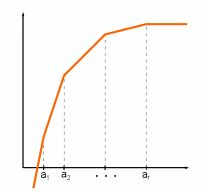
\includegraphics{./figures/L2.2}
  \caption{}
  \end{figure}
\end{nthm}

Any $f(\mathbf{x}) \in \overline\R [x_1, \dots, x_n]$ is the minimum of a load of finite number of affine functions. Then we define,
\begin{ndefi}[Tropical Zero Set]
  $$ \mathcal{V}(f) := \{\mathbf{a} \in \overline\R^n \,|\, \text{ the miniumu of $f(\mathbf{a})$ is attained by at least two terms}\} $$
\end{ndefi}

\begin{figure}[!ht]
\centering
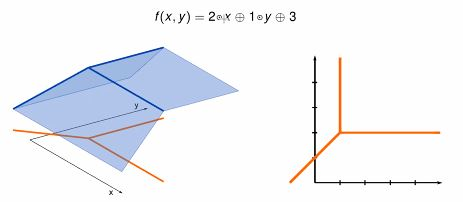
\includegraphics{./figures/L2.3}
\end{figure}

We notice here that instead of points, this time we get some lines where the graph breaks. The tropical zeros are the `bending sets.'\\

\newpage

Now we can consider the following and find the smallest in each region,
\begin{figure}[!ht]
\centering
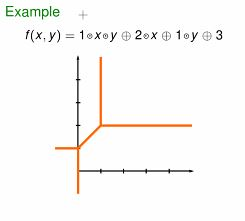
\includegraphics{./figures/L2.4}
\end{figure}

The points where they meet at a point is where they are equal. We have a tropical conic here. Changing the coefficient of the quadratic term from $1 \to -1$ the zero set changes the graph doesn't just flip.\\

Tropical hypersurfaces are `combinatorial' polyhedral complexes with an interesting structure.\\

\subsection{The Tropical Plane}
\begin{minipage}{0.48\textwidth}
  Any two generic tropical lines meets at exactly one point.\\\vspace{30pt}
  \centering
  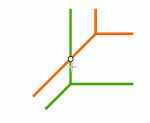
\includegraphics{./figures/L2.5}
\end{minipage}
\begin{minipage}{0.48\textwidth}
  There is unique tropical line going through any two generic points.\\\vspace{30pt}
  \centering
  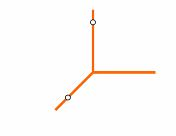
\includegraphics{./figures/L2.6}
\end{minipage}

\begin{minipage}{0.48\textwidth}
  Five points make a conic.\\\vspace{30pt}
  \centering
  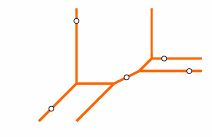
\includegraphics{./figures/L2.7}
\end{minipage}
\begin{minipage}{0.48\textwidth}
  There are no parallel lines in the tropical world. Every collection of lines always intersect once.\\\vspace{30pt}
  \centering
  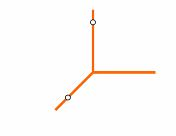
\includegraphics{./figures/L2.6}
\end{minipage}

\newpage
\subsection{Why Tropical Geometry}
Let $K$ be an algebraically closed field with a valuation map: $\text{val}: K \to \overline\R$, that is,
$$ \val(a \cdot b) = \val a \odot \val b \quad \val (a + b) \ge \val a \odot \val b \quad \val a = \infty \iff a = 0  $$

\begin{ndefi}[Trivial Valuation]
  $$ \val x = \begin{cases}
    0 & \text{if $x\ne 0$ }\\
    \infty & \text{otherwise}
  \end{cases} $$
\end{ndefi}

\begin{eg} Here are some fields with evaluations,\\
  \begin{itemize}
    \item Let $K = \C$ and with the trivial evaluation.
    \item $K = \overline\Q$ with the p-adic evaluation.
    \item $K = \C\{\{t\}\}$ the field of Pulseux series; a formal power series of the form,
    $$ a = c_0t^{r_0} + c_1t^{r_1} + \dots + c_kt^{r_k} + \dots$$
    with $c_i \in \C$ and $r_0 < r_1 < \dots$ rational numbers with a common denominator and valuation $\val a = r_0$.
  \end{itemize}
\end{eg}

\noindent
One can tropicalise any $F \in K[x_1, \dots, x_n]$ to $\trop(F) \in \overline\R [x_1] $ by substituting,
$$ + \to \oplus \quad \cdot \to \times \quad f \to \val f $$

\noindent
Suppose $V$ be the zero locus of an ideal $J \subset K[x_1, x_2, \dots, x_n]$. Consder an ideal,
$$ \trop(J) := \langle \trop(F) := F \in J \rangle \subset \overline\R[x_1] $$
The tropicalisation of $V$ is,
$$ \trop := \bigcap_{f \in \trop J} \mathcal{V}(f) $$

\begin{eg}
  Let K= \{\{t\}\} and let $J = \langle x - t \cdot y + q\rangle \subset K[x, y]$ and $V = \{x - t \cdot y + 1 = 0\} \subset K^2$.
  Then we just take the functions and do the tropicalisation,
  \begin{figure}[!ht]
  \centering
  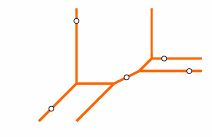
\includegraphics{./figures/L2.7}
  \end{figure}
  and then we get a tropical line. Which is, $\trop V$.
\end{eg}

\newpage
Tropical varieties preseves many invariants of their defining algebraic varieties. It preserves degrees and genus, which is really nice as you can get rid of singularities. We can use the tropicalisation to make sense of some thing yucky and complicated. The tropical degree is the number of rays doing in the imporant directions.\\

\begin{figure}[!ht]
\centering
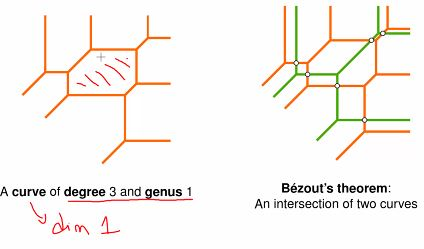
\includegraphics{./figures/L2.9}
\end{figure}


Tropical Geometry has another Bezout's Theorem (which is the same as normal geometry), we can use this with tropical varieties to see the points of intersections. In the diagram above, we have an orange degree 3 and green degree 2 curve. Then we have six intersections.


\begin{ndefi}[Severi Degree]
  The severi degree $N^{d, \delta}$ of $\C\P^2$ is the number of plane curves of degree $d$ and $\delta$ nodal singularities passing through $\frac{(d+3)d}{2}-\delta$ generic points.
\end{ndefi}

\begin{eg}
  \begin{itemize}
    \item $N^{2,0} = $ number of smooth conics through five points. This is one.
    \item $N^{2,1} = $ number of 1-nodal conics through four points. This is three.
    \begin{figure}[!ht]
    \centering
    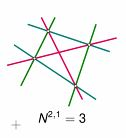
\includegraphics{./figures/L2.10}
    \end{figure}
    \item  $N^{3,1} = $ number of 1-nodal cubics through eight points. This is twelve.
  \end{itemize}
\end{eg}

\begin{nthm}[Mikhalkin 2005]
  Severi degree can be computer tropically
\end{nthm}

\begin{nthm}[Formin-Mikhalkin 2010, conj. Francesco-Itzykson 1994]
  For a fixed $\delta$ thre is a polynomial $N_\delta (d)$ such that for all $d \ge 2\delta$,
  $$ N^{d,\delta} = N_\delta (d) $$
\end{nthm}

\begin{eg} Here are some people that have solved certain values of this problem,
  \begin{itemize}
    \item Steiner 1848: $N^{d,1} = 3(d - 1)^3$
    \item Cayley 1863: $N^{d,2} = \frac{3}{2}(d - 1)(d-2)(3d^2 - 3d - 11)$
    \item Roberts 1867: $\delta = 3$
    \item Vainsencher 1995: $\delta = 4, 5, 6$
    \item Keiman-Piene 2001: $\delta = 7,8$
    \item Block 2010: $\delta = 9, 10, 11, 12, 13, 14$
  \end{itemize}
  \begin{figure}[!ht]
  \centering
  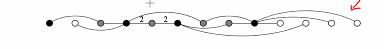
\includegraphics{./figures/L2.11}
  \end{figure}
\end{eg}

Similar approaches have succeeded in the study of Severi degree $N^{\Delta, d}$ of more general toric surfaces, double Hurwitz numbers $H_g(\l, \mu)$, Welshinger invariants $W_d$, ...


\end{document}
